%%%%%%%%%%%%%%%%%%%%%%%%%%%%%%%%%%%%%%%%%%%%%%%%%%%%%%%%%%%%%%%%%%%%%%%%%%%%%%%%%%%%%
% 			Facultad de Ciencias, UAEM.  		Octubre de 2014
% 
%	Alumno: 			Emanuel García Pérez
%	Asginatura:		Procesamiento del Lneguaje Natural
%	Proyecto:		Exposición - Artículo
%	Tema:			"Clasificación de polaridad en textos con opiniones
%					 en español mediante análisis sintáctico de dependencias"
%
%%%%%%%%%%%%%%%%%%%%%%%%%%%%%%%%%%%%%%%%%%%%%%%%%%%%%%%%%%%%%%%%%%%%%%%%%%%%%%%%%%%%%
 

\documentclass{beamer}
 
%\usepackage[spanish,activeacute]{babel}
\usepackage[latin1]{inputenc}
\usepackage{beamerthemeshadow}
\usepackage{graphicx}

\title{\textbf{Clasificaci\'on de polaridad en textos con opiniones en espa\~nol mediante an\'alisis sint\'actico de dependencias}} 
\author{Emanuel Garc\'ia P\'erez}
\date{\today}

\begin{document}

\frame[allowframebreaks]{\titlepage}
\section[Contenidos]{}
\frame{
\transdissolve[duration=0.2]
\tableofcontents
} 

\section{INTRODUCCI\'ON}
\frame{
\transdissolve[duration=0.2]
\frametitle{}
\begin{itemize}
	\item En los \'ultimos a\~nos el alcancen de los blogs, foros y redes sociales han hecho que millones de usuarios los usen para expresar sus opiniones sobre diversos temas.
	\item Esta gran variedad de opiniones y cr\'iticas que abundan en la web son de gran utilidad para que vendedores y fabricantes conozcan el impacto de sus productos en los consumidores.
\end{itemize}
\begin{figure}
  \centering
    
\includegraphics[width=0.5\textwidth]{sentiment1.jpg}
  \label{fig:ejemplo}
\end{figure}
}

\frame{
\transdissolve[duration=0.2]
\frametitle{}
Debido a las ventajas que presenta toda esa informaci\'on y la complejidad que conlleva su an\'alisis es necesario la b\'usqueda de soluciones eficientes capaces de monitorizar este flujo de informaci\'on. La miner\'ia de opini\'on(MO) se enfoca en el tratamiento autom\'atico de informaci\'on con opini\'on, lo que permite extraer la polaridad(positiva, negativa, neutra, mixta) de un texto.
}


\section{ESTADO DEL ARTE}
\frame{
\transdissolve[duration=0.2]
\frametitle{Polaridad en textos}
La clasificaci\'on de la polaridad en textos es un problema de gran relevancia en la MO, este ha sido abordado desde dos enfoques:
\begin{itemize}
	\item Concebir esta tarea como un proceso gen\'erico de clasificaci\'on, y a partir de un conjunto de datos de entrenamiento, donde los textos son anotados con su respectiva polaridad, se construye un clasificador mediante aprendizaje autom\'atico(AA).
	\item Apoyarse en la orientaci\'on sem\'antica(OS) de las palabras, cada t\'ermino que expresa opini\'on es anotado con un valor que representa su polaridad.
\end{itemize}
}

\frame{
\transdissolve[duration=0.2]
\frametitle{Sistemas de MO}
La mayor\'ia de los sistemas de MO existentes se enfocan en tratar \'unicamente textos en ingles. Para textos en espa\~nol el, quiz\'as, sistema m\'as relevante es "The Spanish SO Calculator", desarrollado en la universidad Simon Fraser de Canad\'a.
}


\frame{
\transdissolve[duration=0.2]
\frametitle{Spanish SO CA}
\begin{itemize}
	\item Resuelve la OS almacenada a nivel individual en: adjetivos, sustantivos, verbos y adverbios.
	\item Trata modificadores de la polaridad, como la negaci\'on o intensificadores("muy", "poco", "bastante").
	\item Detecta y excluye el sentimiento reflejado en el contenido no f\'actico del texto(expresiones condicionales o subjuntivas.)\\
	La forma m\'as com\'un de tratar estas construcciones ling\"uisticas es a nivel l\'exico, y "The Spanish SO CA" no es la excepci\'on.
\end{itemize}
}

\frame{
\transdissolve[duration=0.2]
\frametitle{Negaci\'on}
Respecto a la negaci\'on tenemos lo siguiente: 
\begin{itemize}
	\item Taboada, 2011: utiliza informaci\'on morfol\'ogica para identificar el alcance dela negaci\'on.
	\item Yang, 2008: considera el alcance de la negaci\'on como los t\'erminos a la derecha de la negaci\'on.
	\item Fern\'andez Anta, 2012: se emplea una heur\'istica que asume que los tres elementos a continuaci\'on de una negaci\'on son los que deben cambiar su polaridad.
\end{itemize}
}

\frame{
\transdissolve[duration=0.2]
\frametitle{Intensificaci\'on}
Para los intensificadores tenemos: 
\begin{itemize}
	\item Fern\'andez Anta, 2012: considera de nuevo que los tres t\'erminos a la derecha son los que deben variar su polaridad.
	\item Taboada, 2011: adem\'as de los intensificadores propiamente dichos, trata como tales aspectos del discurso como la conjunci\'on "pero" o las may\'usculas.
\end{itemize}
}

\frame{
\transdissolve[duration=0.2]
\frametitle{}
La propuesta utilizada se basa en obtener la estructura sint\'actica del texto para tratar las construcciones ling\"uisticas e identificar los elementos de la frase que est\'an implicados en ellas.\\ Trabajos anteriores(Jiu, yuMeng, 2009) han mostrado los beneficios de utilizar la estructura sint\'actica de la frase en textos con ocurrencias de t\'erminos negativos. 
}

\frame{
\transdissolve[duration=0.2]
\frametitle{}
Otro problema que enfrentan los sitemas de MO es la calidad ortogr\'afica de los textos. Si estos provienen de la web, se debe tener en cuenta que a menudo sus autores omiten acentos, letras, vocablos, etc., o utilizan abreviaturas no reconocidas y oraciones agram\'aticales.\\ La soluci\'on m\'as utilizada es usar patrones heur\'isticos para adaptar el texto.
}


\section{CLASIFICACI\'ON DE OPINIONES BASADA EN DEPENDENCIAS}
\frame{
\transdissolve[duration=0.2]
\frametitle{}
En contraste a las propuestas l\'exicas dominantes, se propone utilizar la estructura sint\'actica de la frase para obtener la OS de un texto. Inicialmente se debe hacer un preprocesamiento de los textos que contemple los siguientes aspectos:
\begin{itemize}
	\item Unificaci\'on de expresiones compuestas que actuan como una sola unidad de significado("a menos que").
	\item Normalizaci\'on de los signos de puntuaci\'on.
\end{itemize}
Posteriormente se debe segmentar el texto en oraciones y tokenizar cada una, para despu\'es hacer el etiquetado morfosint\'actico de cada palabra del texto.
}

\frame{
\transdissolve[duration=0.2]
\frametitle{}
El siguiente paso es realizar el an\'alisis sint\'actico de dependencias para identificar las relaciones binarias "padre/dependiente" entre los t\'erminos de una oraci\'on. Se incluye un elemento inicial(ROOT) para facilitar las definiciones formales e implementaciones. Cada vinculo binario constituye una dependencia, que se anota con la funci\'on sint\'actica que relaciona los dos t\'erminos(\'Arbol de dependencias). Se utilizo el corpus Ancora(Taul\'e, Mart\'i, Recasens, 2008) como referencia para definir las relaciones de dependencia.
\begin{figure}
  \centering
    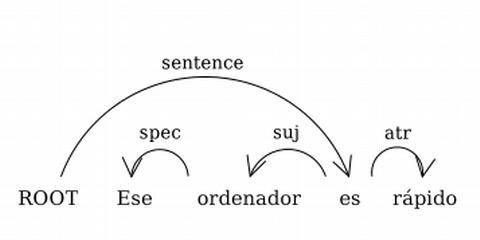
\includegraphics[width=0.5\textwidth]{arbol1.jpg}
  \label{fig:ejemplo}
\end{figure}
}

\frame{
\transdissolve[duration=0.2]
\frametitle{}
Finalmente para realizar el an\'alisis sem\'antico, se utiliza SODcitionariesV1.11Spa(Brooke, Tofiloski, Taboada, 2009), un conjunto de diccionarios de polaridad para adjetivos, sustantivos, verbos, adverbios e intensificadores. Cada t\'ermino tiene asociado un valor entre -5 y 5, siendo -5 lo m\'as negativo y 5 lo m\'as positivo. El valor asignado a cada palabra corresponde con una OS gen\'erica, independientemente del dominio o contexto donde se use.
}

\frame{
\transdissolve[duration=0.2]
\frametitle{}
Ej: r\'apido(adj):= 2, recomendar(verb):= 2
\begin{figure}
  \centering
    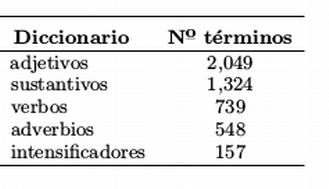
\includegraphics[width=0.5\textwidth]{tabla1.jpg}
  \label{fig:ejemplo}
\end{figure}
Los valores numericos asociados a los intensificadores tiene un significado distinto, representan el porcentaje(positivo o negativo) por el que modifican el sentimiento de la expresi\'on a la que afectan.
}


\subsection{Propuesta Base}
\frame{
\transdissolve[duration=0.2]
\frametitle{}
Se determina la polaridad de un texto a partir de la combinaci\'on de la OS de sustantivos, adjetivos, verbos, y adverbios, sin considerar la estructura sint\'actica del texto(construcciones ling\"uisticas complejas).
}


\subsection{Tratamiento de la Intensificaci\'on}
\frame{
\transdissolve[duration=0.2]
\frametitle{}
Los intensificadores son t\'erminos o expresiones que modifican la polaridad de ciertas palabras. Podemos clasificarlos en dos tipos:
\begin{itemize}
	\item Amplificadores: permiten aumentar la polaridad; ("muy", "bastante").
	\item Decrementadores: permiten disminuir la polaridad; ("poco", "en absoluto").
\end{itemize}
Para modelar esta construcci\'on, se asocia a cada intensificador un factor de ponderaci\'on. Se utiliza el \'arbol de dependencias para determinar la parte de la frase que se ve afectada por tal modificaci\'on, considerando las dependencias anotadas en Ancora. 
}

\frame{
\transdissolve[duration=0.2]
\frametitle{}
Si hay varios intensificadores presentes, se combinan sus porcentajes de intensificaci\'on antes de que actuen sobre el t\'ermino afectado. \\
Ej: "muy":= 0.25, "en absoluto":= -1 \\
"muy r\'apido"|OS: 2*(1+0.25) = 2.5\\
"en absoluto muy r\'apido"|OS: 2*(1+(-1+0.25)) = 0.5
}


\subsection{Tratamiento de las oraciones adversativas}
\frame{
\transdissolve[duration=0.2]
\frametitle{}
Los nexos adversativos contraponene hechos expresados en dos oraciones. En MO este tipo de frases se emplean para restringir o excluir opiniones, que puede ser considerado como un caso especial de intensificaci\'on.\\
Un \'arbol de dependencias permite identificar con precisi\'on la oraci\'on subordinada y la subordinante.
}

\frame{
\transdissolve[duration=0.2]
\frametitle{}
El corpus Ancora representa sint\'acticamente este tipo de oraciones de forma diferente seg\'un el nexo concreto, se opto por hacer enfoque en los nexos m\'as relevantes que Ancora representa de manera uniforme; siendo estos divididos en dos grupos:
\begin{itemize}
	\item Restrictivos: reducen la OS de la oraci\'on principal. Destaca la conjunci\'on "pero".
	\item Excluyentes: eliminan por completo lo expresado en la primera oraci\'on; "sino".
\end{itemize}
}

\frame{
\transdissolve[duration=0.2]
\frametitle{}
Seg\'un la clase del nexo, se pondera el sentimiento acumulado, tanto en la oraci\'on subordinante y la subordinada, de forma distinta.\\
Para homogenizar la estructura sint\'actica de otras subordinadas adversativas y simplificar la ponderaci\'on de estas oraciones, se opto por reestructurarlas en el \'arbol de dependencias. Se cre\'o un nuevo tipo de dependencia, art\_rel\_adversative, para identificar sint\'acticamente el inicio de una cl\'ausula de este tipo.
}


\subsection{Tratamiento de la Negaci\'on}
\frame{
\transdissolve[duration=0.2]
\frametitle{}
Muchos t\'erminos o expresiones permiten negar una opini\'on, la distinci\'on de un negador y un intensificador decrementador suele ser difusa. Se restringio el tratamiento de esto a los t\'erminos "no", "nunca" y "sin". Expresiones negadoras como "lo menos" o "en absoluto" fuer\'on tratadas como intensificadores, se uso la informaci\'on sem\'antica de SODictionariesV1.11Spa para este tipo de locuciones.\\
Para resolver el sentimiento de una oraci\'on con t\'erminos negativos se necesitan dos pasos:
\begin{itemize}
	\item Identificar el alcance de la negaci\'on.
	\item Modificar la polaridad del fragmento de la oraci\'on correspondiente.
\end{itemize}
}


\subsubsection{Identificaci\'on del alcance de la negaci\'on}
\frame{
\transdissolve[duration=0.2]
\frametitle{}
En primer lugar se establece un alcance candidato, formado por el padre del negador y sus hermanos, despu\'es se corrige ese alcance aplicando las siguientes reglas:
\begin{enumerate}
\item Regla del padre subjetivo: si el padre del negador aparece en los diccionarios sem\'antico, entonces solo \'el constituye el alcance corregido de la negaci\'on.
\item Regla del atributo o complementeo directo: si alguno de los hermanos desempe\~na una de estas funciones sint\'acticas, entonce dicho hermano forma parte del alcance de la negaci\'on.
\item Regla del complemento circunstancial m\'as cercano: si alguna rama al mismo nivel del negador actua como complemento circunstancial, entonces dicha rama forma el alcance corregido. En caso de varios complementos circunstanciales, solo se incorpora el m\'as cercano f\'isicamente al negador.
\end{enumerate}
}

\frame{
\transdissolve[duration=0.2]
\frametitle{}
Si ninguna de las reglas se cumple, entonces se asume el alcance candidato(salvo el nodo padre) como el corregido.
}

\subsubsection{Modificaci\'on de la polaridad}
\frame{
\transdissolve[duration=0.2]
\frametitle{}
Una vez obtenido el alcance corregido de la negaci\'on, se extrae su polaridad y despu\'es el valor obtenido es modificado en una cantidad preestablecida de signo contrario.
}


\section{RESULTADOS EXPERIMENTALES}
\subsection{Implementaci\'on}
\frame{
\transdissolve[duration=0.2]
\frametitle{}
Se realizo la implementaci\'on en Python usando el toolkit NLTK, para la etiquetaci\'on se aplico el algoritmo de Brill utilizando el corpus Ancora para el entrenamiento(90\% del corpus para entrenar y el 10\% restante para evaluar).\\ Para mejorar el rendimiento practico del etiquetador para textos de la web, el fragmento del corpus para el aprendizaje fue ampliado para que cada oraci\'on tuviese un equivalente si acentos gr\'aficos. El an\'alisis sint\'actico de dependencias se realizo con el algoritmo Nivre arc-eager(Nivre, 2008) generado con Malt-Parser mediante AA a partir del corpus Ancora.
}

\frame{
\transdissolve[duration=0.2]
\frametitle{}
Un problema a tener en cuenta, fue solventar la mayor importancia que suelen tener las oraciones finales de una opini\'on. Para modelar esto, se opto por aumentar 75\% la OS de las 3 \'ultimas  frases de una cr\'itica.\\
Otro problema, de la tendencia positiva del lenguaje, es expresar una opini\'on negativa usando negaciones de t\'erminos positivos, "no barato", "no bueno", para compensar esta desviaci\'on muchas aproximaciones l\'exicas incrementan la OS de los t\'erminos negativos. Se mejoro la presici\'on del sistema aumentando la dispenrsi\'on de la OS un 20\%, haciendo que las polaridades sean entre -6 y 6.
}


\subsection{Evaluaci\'on}
\frame{
\transdissolve[duration=0.2]
\frametitle{}
Para la evaluaci\'on se empleo un corpus formado por 400 documentos; SFU Spanish Review Corpus(Brooke, Tofiloski, Taboada, 2009). Contiene rese\~nas de productos y servicios de ocho categor\'ias: lavadoras, hoteles, pel\'iculas, coches, ordenadores, libros, m\'usica y moviles.\\
Cada categor\'ia dispone de 50 documentos, 25 expresan una opini\'on positiva y 25 una negativa. Se procesa cada texto y se obtiene la OS, si es mayr a 0 es positiva y es negativa en caso contrario.
}

\frame{
\transdissolve[duration=0.2]
\frametitle{}
Las construcciones ling\"uisticas tratadas han mejorado el rendimiento, el incremento obtenido al incorporar la negaci\'on es muy significativo.
\begin{figure}
  \centering
    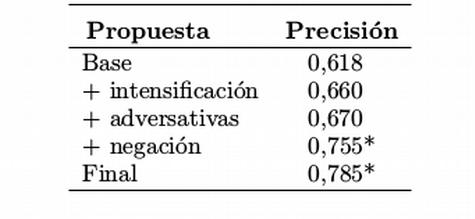
\includegraphics[width=0.5\textwidth]{tabla2.jpg}
  \label{fig:ejemplo}
\end{figure}
Se realizar\'on pruebas chi-cuadrado(p $<$ 0.01), comparando con las polaridades correctas.
}

\frame{
\transdissolve[duration=0.2]
\frametitle{}
Haber utilizado el mismo corpus y los mismos diccionarios sem\'anticos, permite comparar esta alternativa sint\'actica con la soluci\'on l\'exica.\\
Hubo un incremento en el rendimiento respecto a "The Spanish SO-CA", tambi\'en se creo un clasificador SVM, basado en AA, usando WEKA.
\begin{figure}
  \centering
    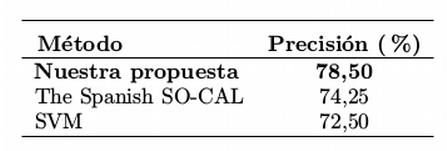
\includegraphics[width=0.5\textwidth]{tabla3.jpg}
  \label{fig:ejemplo}
\end{figure}
}

\end{document}